% Innehållet i Vasungavisor 2010
%
% Kapitel "I Högan Nord"

\songchapter{I Högan Nord}
\chapterimage[width=8cm]{../bilder/i_hogan_nord.png}

% Innehållet i Vasungavisor 2018
%
% Sången "Vårt Land"

\beginsong{Vårt land}[
  by={Johan Ludvig Runeberg},
  index={Finlands nationalsång}]  
  
\beginverse*
Vårt land, vårt land, vårt fosterland,
ljud högt, o dyra ord!
Ej lyfts en höjd mot himlens rand,
ej sänks en dal, ej sköljs en strand,
mer älskad än vår bygd i nord,
än våra fäders jord.
\endverse

\beginverse*
Din blomning, sluten än i knopp,
skall mogna ur sitt tvång.
Se, ur vår kärlek skall gå opp,
ditt ljus, din glans, din fröjd, ditt hopp.
Och högra klinga skall en gång
vår fosterländska sång.
\endverse
\endsong

\sclearpage
% Innehållet i Vasungavisor 2018

\beginsong{Vasa marsch}[
  by={Zacharias Topelius},
  index={I högan nord vår vagga stod}]
  
\beginverse*
I högan nord vår vagga stod
vid stormigt hav och skummig flod.
Vi växte upp ur frostig bädd
som vintergran i drivor klädd.
Han står så grön i vita snön,
han reser stark sin kronas park
ur armod och ur ödemark.
\endverse

\beginverse*
Som tusen vågor sammangå
kring Finlands bygd i gördel blå,
så mötas hjärtan, mötas namn,
o, fosterland, uti din famn.
Att bära glatt din fanas skatt,
att kämpa med i främsta led
var fäders bragd, var Vasa sed.
\endverse

\beginverse*
Vårt land! Vårt finska fosterland!
Din fasta botten är vår strand.
Så lär oss bli din starka vall,
som havets våg ej bryta skall.
Slå högt, vår barm! Väx stark, vår arm!
Väx stor i skygd av söners dygd,
vår höga nord, vår finska bygd!
\endverse
\endsong
\sclearpage
% Innehållet i Vasungavisor 2018

\beginsong{Vaasan marssi}[
  by={A Noponen},
  index={Miss' laaja aukee Pohjanmaa}]
  
\beginverse*
Miss' laaja aukee Pohjanmaa,
veet merten, virtain vaahtoaa,
me siellä maassa hallojen
niin kasvoimme kuin kuuset sen:
ei niitä sää voi säikyttää,
ei kuihtumaan saa talvetkaan,
ei puute kurjuus korpimaan.
\endverse

\beginverse*
Kuin aallot järvein tuhanten
käy rannoillamme yhtehen,
niin liittohon myös meidät saa
sun nimes', kallis synnyinmaa.
Jos vainomies sun sulkis' ties',
niin kuolemaan me taistellaan
kuin Vaasan urhot ainiaan.
\endverse

\beginverse*
Et turvatta sa, Suomi, jää,
on vankka Pohjas' ranta tää,
ja muuris' meidän olla suo,
jot' eivät myrskyt maahan luo.
Pois unteluus ja hervakkuus!
Niin onnehen maan pohjaisen
vie kunto, työ sen poikien.
\endverse
\endsong
\sclearpage
\input{KymmenenVirranMaa.tex}
\sclearpage
% Innehållet i Vasungavisor 2018

\beginsong{Österbotten, Österbotten}[
  by={Gånge Rolf}]

\beginverse*
Österbotten, Österbotten,
land vi ha ändå!
Allt från Tornes dubbelälvar
ner till Lappfjärds å.
Le i ljusa sommarnätter,
åkrar, ängar, fjäll och slätter,
skogar, sjöar, skär och öar,
bottenböljor blå.
\endverse

\beginverse*
Österbotten, Österbotten,
hem för frihet, rätt!
Hellre dö än bojor bära,
det var fädrens sätt.
Aldrig de sin rygg ha buktat,
våld och väld de själva tuktat.
Stolta minnet, elde sinnet
än hos bottnisk ätt!
\endverse
\endsong
\begin{intersong}
	\begin{center}
		\includegraphics[height=25mm]{../bilder/sad.jpg} 
	\end{center}
\end{intersong}
\sclearpage


\beginsong{Marsch för UV}[
by={Gånge Rolf},
index={Fri såsom Bottens brusande bölja},
]

\beginverse*
Fri såsom Bottens brusande bölja
växte vår unga, vår trotsiga håg,
älskar som hon med kärlek omskölja
stränder och öar, där dagen han såg.
/: Vill dock ej ständigt vid stranden förbida,
ut vill han, ut för att kämpa och strida,
ut på de blånande fjärdarna vida,
världen omkring uppå vikingatåg. :/
\endverse

\beginverse* 
Emot mörker, emot fördom, går okuvlig den
bottniska fylkingen fram
för att skapa en framtid åt sig själv, 
åt sin hembygd, sitt språk och sin stam. 
/: Var kämpens bana gått, 
hur han sin strid bestått,
hem han längtar dock sist till sin älskade kust
att som vågen lugn i hågen somna bort från
levnadens stormiga dust. :/
\endverse
\endsong



\sclearpage


\beginsong{Björneborgarnas marsch}[
by={Johan Ludvig Runeberg},
index={Söner av ett folk som blött}]

\beginverse*
Söner av ett folk som blött
på Narvas hed, på Polens sand, på Leipzigs slätter, Lützens kullar,
än har Finlands kraft ej dött,
än kan med oväns blod ett fält här färgas rött.
Bort, bort, vila, rast och fred!
En storm är lös, det ljungar eld och fältkanonens åska rullar;
framåt, framåt led vid led!
På tappre män se tappre fäders andar ned.
Ädlaste mål
oss lyser på vår bana;
skarpt är vårt stål
och blöda är vår vana.
Alla, alla käckt framåt!
Här är vår sekelgamla frihets sköna stråt.
Lys högt, du segersälla fana,
sliten av strider sen en grånad forntids dar,
fram, fram, vårt ädla, härjade standar!
Än finns en flik med Finlands gamla färger kvar!
\endverse
\endsong

\begin{intersong}
	\begin{center}
		\includegraphics[scale=.24]{../bilder/bjorneborgarnas_marsch.png} 
	\end{center}
\end{intersong}
\sclearpage
\input{ModersmaletsSang.tex}
\sclearpage
\input{FinlandiaHymnen.tex}
\sclearpage


\beginsong{En sommardag i Kangasala}[
by={Zacharias Topelius},
index={Jag gungar i högsta grenen},
]

\beginverse*
Jag gungar i högsta grenen
 av Harjulas högsta ås.
Vitt skina de blåa vatten, 
så långt de av ögat nås.
Av Längelmävesis fjärdar där skimrar ett silverband
och Roines älskliga vågor i fjärran kyssa dess strand,
och Roines älskliga vågor i fjärran kyssa dess strand.
\endverse

\beginverse*
Och blå som en älsklings öga 
och klar som ett barndomshem
den gungande Vesijärvi 
sig stilla smyger till dem. 
Och hundrade öar simma allt uti dess vida famn,
naturens gröna tankar i blåa vågornas hamn,
naturens gröna tankar i blåa vågornas hamn.
\endverse

\beginverse*
Du helige himlens Herre, 
hör lilla fågelns bön! 
Ack, hur är din jord så ljuvlig, 
ack, hur är din himmel så skön! 
O låt våra sjöar stråla
klart uti vår kärleks brand! 
O herre, lär oss att älska, o lär oss att älska vårt land! 
O herre, lär oss att älska, o lär oss att älska vårt land!
\endverse
\endsong



\sclearpage

\beginsong {Vid en källa}[
by={Johan Ludvig Runeberg},
index={Jag sitter, källa, vid din rand}]

\beginverse*
Jag sitter, källa, vid din rand 
Och ser på molnens tåg.
/: Hur ledda av en osedd hand 
de växla i din våg.:/
\endverse

\beginverse* 
Där kom en sky, den log så röd, 
som rosenknoppen ler.
/: Men ack hur snart farväl den bjöd, 
för att ej komma mer.:/
\endverse

\beginverse* 
Dock, där en annan mera klar 
och strålande igen. 
/: Ack, lika flyktig, lika snar, 
försvinner även den.:/
\endverse

\beginverse
Jag tänker, när jag ser dig så, 
uppå min egen själ.
/: Hur mången gyllne sky också 
har bjudit den farväl.:/
\endverse

\beginverse* Men hur de kommit, hur de gått,
jag känt dem ganska väl. 
/: De varit tomma skyar blott
i spegeln av min själ.:/
\endverse
\endsong



\sclearpage


\beginsong{Sommarmarsch}[
by={Ernst V. Knape},
index={Över bygden skiner sol},
]

\beginverse*
Över bygden skiner sol i blånande sky'
och när sunnan kring fälten dansar,
klöverns kransar
sprida sin sommardoft
till alla loft
i grönklädd by.
\endverse

\beginchorus
/: Och det vajar i björkar och leker i lid'
och det susar av sånger i sommarns glada tid'
Signe Gud den dofterika sommartid.:/
\endchorus							% Sluta refräng

\beginverse* 
Och med vännen vill jag vandra hand uti hand,
vill jag vandra bland blomsterängar,
klöversängar,
vandra i solens sken
på åkerns ren
till älvens strand,
\endverse

\beginchorus
/: där det vajar i björkar och leker i lid'
där det susar av sånger i sommarns glada tid.
Signe Gud den glädjerika sommartid.:/
\endchorus	
\endsong



\sclearpage
\input{MuIsamaa.tex}
\sclearpage


\beginsong{Du gamla, du fria}[
by={Richard Dybeck},
index={Sveriges nationalsång},
]

\beginverse*
 Du gamla, du fria, du fjällhöga Nord,
du tysta, du glädjerika sköna!
Jag hälsar dig, vänaste land uppå jord,
/: din sol, din himmel, dina ängder gröna.:/
\endverse

\beginverse*
Du tronar på minnen från fornstora dar, 
då ärat ditt namn flög över jorden.
Jag vet, att du är och du blir vad du var.
/: Ja, jag vill leva, jag vill dö i Norden.:/
\endverse
\endsong



\begin{intersong}
\begin{center}
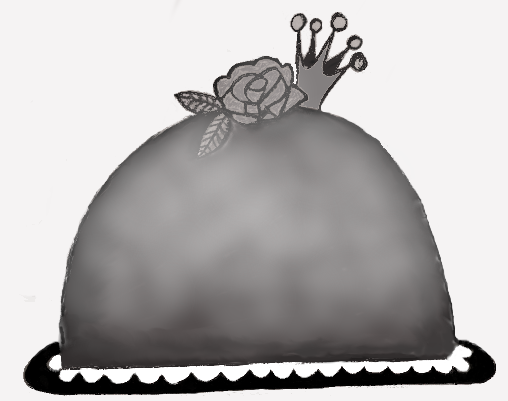
\includegraphics[width=1\textwidth]{../bilder/fardigabilder/CamillasFardigaBilder/Sverigesnationalsangprincesstarta.png} 
\end{center}
\end{intersong}
\sclearpage
\input{DerErEttYndigtLand.tex}
\begin{intersong}
	\begin{center}
		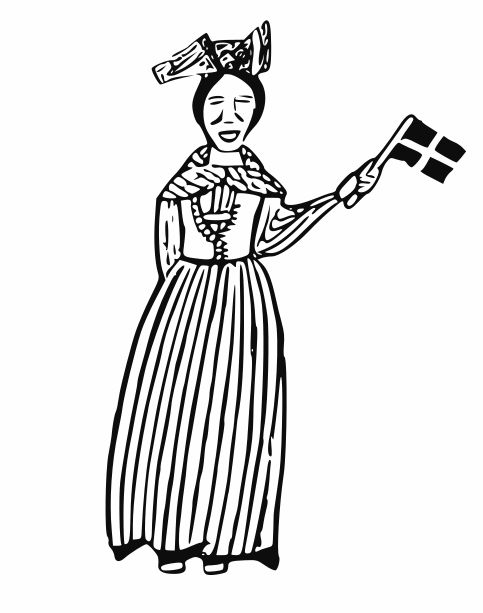
\includegraphics[width=4cm]{../bilder/fardigabilder/Danmarksnationalsng.png} 
	\end{center}
\end{intersong}


\sclearpage

\beginsong {Ja, vi elsker dette landet}[
by={Bjørnstjerne Bjørnson}]

\beginverse*
Ja, vi elsker dette landet,
som det stiger frem,.
furet, værbitt over vannet,
med de tusen hjem.
Elsker, elsker det og tenker
på vår far og mor
og den saganatt som senker
drømme på vår jord.
Og den saganatt som senker,
senker drømme på vår jord.
\endverse
\endsong

\begin{intersong}
	\begin{center}
		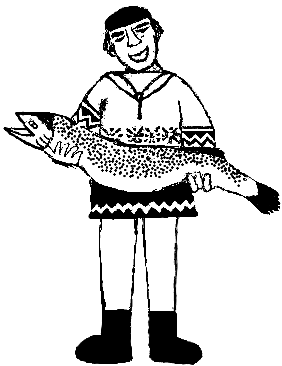
\includegraphics[width=0.55\textwidth]{../bilder/fardigabilder/CamillasFardigaBilder/Norgesnationalsang2.png} 
	\end{center}
\end{intersong}




\sclearpage
